\section{\texttt{googleVis}}

% ----------------------------------------------------------------------

\subsection{Descrição}

\begin{frame}

  Funções R para gráficos \textit{a la}
  \href{https://developers.google.com/chart/interactive/docs/gallery}{
    Google Docs SpreadSheets}.  \vspace{2em}

  \begin{itemize}
  \item Autores: Markus Gesmann, Diego de Castillo, Joe Cheng
  \item Lançamento: 03-Dec-2010
  \item Versão: 0.5.9
  \item URL:
    \url{http://cran.r-project.org/web/packages/googleVis/index.html},
    \url{https://github.com/mages/googleVis}
  \end{itemize}
  
\end{frame}

\begin{frame}

  \begin{columns}
    \column{0.5\linewidth}
    \begin{itemize}
    \item O mais conhecido: \textbf{Motion Chart}, popularizado por Hans
      Rosling em seu
      \href{https://www.ted.com/talks/hans_rosling_shows_the_best_stats_you_ve_ever_seen}{TED
        talk}.
    \item Visualizar dados em data frames com gráficos Google sem upload
      no Google Docs.
    \item O resultado é um html com funções JavaScript hopedadas pelo
      Google que é rederizado pelo navegador.
    \item Requer conexão, às vezes flash.
    \end{itemize}

    \column{0.49\linewidth}
    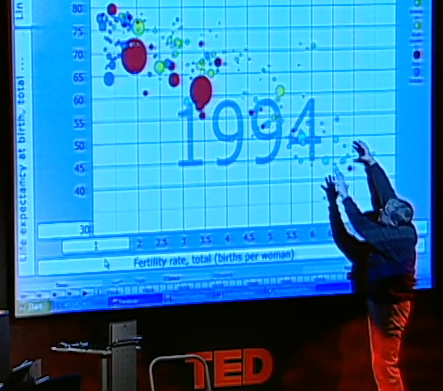
\includegraphics[width=\linewidth]{./images/ted-hans-hosling.png}
  \end{columns}

\end{frame}

\begin{frame}
  \begin{itemize}
  \item Dado estruturado em \texttt{DataTable}.
  \item Transforma \texttt{data.frame}s em objetos JSON.
  \item Usa o \texttt{RJSONIO} para gerar JSON.
  \end{itemize}

  \begin{center}
    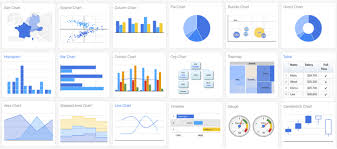
\includegraphics[width=0.5\linewidth]{./images/googleVis.jpg}
  \end{center}

\end{frame}

% ----------------------------------------------------------------------

\subsection{Como usar}
  
\frame{
  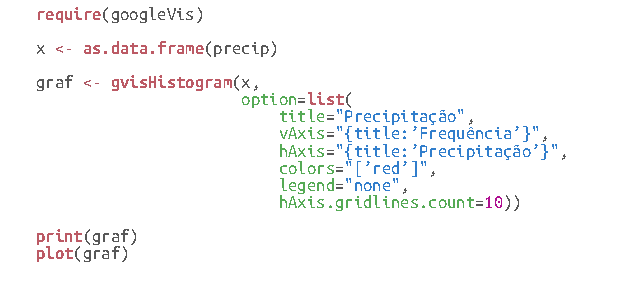
\includegraphics{./tikz/googleVis_gvisHistogram-1.pdf}
}

\frame{
  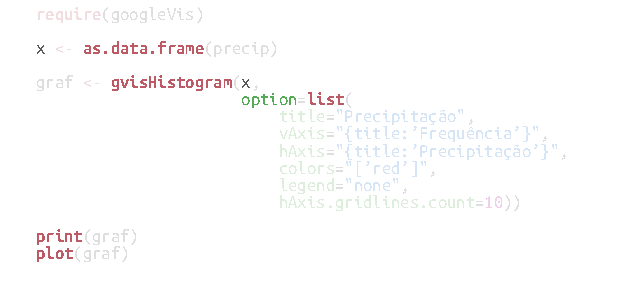
\includegraphics{./tikz/googleVis_gvisHistogram-2.pdf}
}

\frame{
  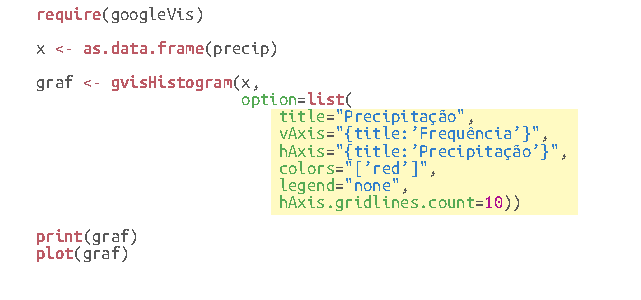
\includegraphics{./tikz/googleVis_gvisHistogram-3.pdf}
}

% ----------------------------------------------------------------------

\subsection{Exemplos}

\begin{frame}

  \todo{Incluir exemplos de ce064}

  Praticando:
  \begin{enumerate}
  \item \href{run:./R/googleVis/googleVis.R}{R Script googleVis}
  \end{enumerate}

  \vspace{0.5cm} Algumas aplicações com o googleVis:
  \begin{itemize}
  \item
    \href{http://cran.r-project.org/web/packages/googleVis/vignettes/}{
      Galeria do autor}
  \item \href{http://www.r-bloggers.com/?s=googleVis}{Busca no R
      Bloggers}
  \end{itemize}

\end{frame}
